\chapter{Architecture}

This chapter describes the architecture of JPaxos.
First the general architecture of the library is presented, consecutively focusing on its parts in detail.
Later the most significant data structures and threading architecture details are presented.

\section{Architecture overview}
\indent\par
Easiest way to understand the architecture of JPaxos is to analyze it's architecture in top-down approach.

\subsection{Processes and their communication}

For JPaxos there are two possible approaches of building replicated services. The first, recommended by us, requires from the service client application using a \texttt{Client} module. The other approach incorporates client module with replica, but it places the responsibility for finding a working replica on the user. The possible approaches are visualised on figure \ref{fig:jpaxos_processes}.

\begin{figure}[h]
 \begin{tabular}{ccc}
  
\includegraphics[width=0.44\textwidth]{architecture/userArchitecture1.pdf}
  &
  \hspace{0.02\textwidth}
  &
  
\includegraphics[width=0.44\textwidth]{architecture/userArchitecture2.pdf}
  \\ 
  \scriptsize a) JPaxos client integrated with service client
  & & 
  \scriptsize b) JPaxos client integrated with the replica\\
 \end{tabular}
 \fcmfcaption{Two models of JPaxos}\label{fig:jpaxos_processes}
\end{figure}

The JPaxos \texttt{Client} is responsible for connecting to replicas, providing availability of service as the replica connected with client crashes and ensures that the request will be eventually answered.

Integrating the \texttt{Client} module with service client provides full transparency of replication for the clients.
The service client contacts with the JPaxos \texttt{Client} module as if it would contact with the service -- i.e. it executes requests and gets answers for them.

If one chooses the second approach -- integrating \texttt{Client} in the replica -- the transparency is lost, and the programmer using JPaxos must care for selecting a working replica himself. However, this approach enables using JPaxos in wider context -- for example, one could possibly create a REST web service, and use an usual web client as the service Client, while the service itself would be replicated using JPaxos.

The JPaxos Replica module is responsible for global request ordering, passing the requests to the service, answering to the clients and recovering service from crash.

The service itself must be integrated within JPaxos replica. It gets the requests and responds to them. However, in order to make the resource usage bounded JPaxos requires additional functionality from the service, that partially breaks the transparency - the service must provide snapshots of it's state
once a time, % TODO: lepsze sformuowanie
as well as be able to recover it's state from a snapshot, possibly made by other replica.
As we assume that the services are deterministic, recovering from snapshot originating from other replica is not an issue, however for some services creating a snapshot may present a challenge.

\subsection{Client and client-replica communication}

The JPaxos client module is a single, small-weight module that performs several tasks:
\begin{itemize} 
 \item Connects to the replicated service
 \item Reconnects to the replicated service if the connection is lost (e.g. if a replica crashed)
 \item Retrieves (or acknowledges) a Client ID for recognising the requests
 \item Sends the requests
 \item Waits for answer, retransmitting the request if needed
\end{itemize}

For the communication with replicas Client uses TCP protocol.

\subsection{Service}

Service is the core part -- in fact it's the service that uses JPaxos for replication.
In order to connect a service with the library, it must implement an interface provided by JPaxos. The interface provides required communication between the library and the service.

The interface for interconnecting JPaxos replica and service allows for:
\begin{itemize}
 \item Executing requests and providing answers for them
 \item Creating Snapshots
 \item Recovering from snapshots
\end{itemize}

\subsection{Replica}

Replica is the most important part of the JPaxos. It consists of numerous modules as depicted on the figure \ref{fig:replica_architecture}.

\begin{figure}[h]
 \centering
 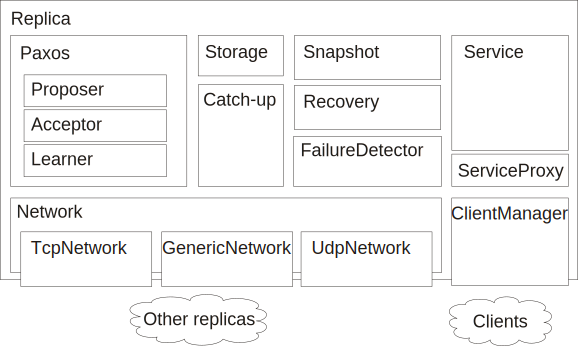
\includegraphics[keepaspectratio, width=0.75\textwidth]{architecture/replica_architecture.pdf}
 \caption{Block diagram of JPaxos modules}
 \label{fig:replica_architecture}
\end{figure}

Short description of the modules of JPaxos goes as follows:

\begin{description}
  \item[Replica ] interconnects other modules - especially the ClientManager, Paxos ans ServiceProxy
  \item[ClientManager ] maintains connection to clients, receives requests from them and forwards the answers
  \item[Paxos ] implements Paxos consensus algorithm
  \begin{description}
    \item[Proposer ] sends new proposes
    \item[Acceptor ] receives proposes and accepts them
    \item[Learner ] collects accepts and decides
  \end{description}
  \item[CatchUp ] takes care for lost ballots as well as retrieves the state from others on recovery
  \item[SnapshotMaintainer ] controls snapshot mechanism
  \item[Recovery ] chooses proper recovery method and does the actual recovery processes
  \item[Storage ] keeps the state of Paxos protocol - view number, log of consensus instances and snapshot
  \item[Service Proxy ] as only module contacts with the Service, provides as much transparency as possible for the service
\end{description}

\section{Storage and data structures}
\label{sec:storage_and_data_structures}

Apart of modules and interaction among them it is important to choose proper routines to access data. Both within modules as well as data shared across whole JPaxos.

\subsection{Process descriptor}

Every application has some configurable options that stay constant during the run. In JPaxos all these constants are kept in the \texttt{ProcessDescriptor} class.

During the startup JPaxos reads configuration file and initializes ProcessDescriptor with:
\begin{tightList}[\setlength{\labelwidth}{0em}]
 \item[\textbf{crashModel}] the crash model (see chapter \ref{chapter:recovery})
 \item[\textbf{logPath}] path for the stable storage
 \item[\textbf{localId}] the number of replica
 \item[\textbf{numReplicas}] count of the replicas
 \item[\textbf{windowSize}] preferred window size (see \ref{subsec:concurrent_instances})
 \item[\textbf{batchingLevel}] maximum size of the batch (see \ref{sec:batching})
 \item[\textbf{maxBatchDelay}] delay for connecting requests for batching
 \item[\textbf{network}] network protocol to be used
 \item[\textbf{maxUdpPacketSize}] threshold for generic network
\end{tightList}

\subsection{Storage interface}
\label{subsec:storage_interface}

\texttt{Storage} interface is responsible for holding the data for Paxos
protocol.

The data is shared across various modules.
It is very likely that various threads might want to access the Storage simultaneously. In order to prevent concurrency-related errors only one thread, dispatcher, may access these data. So if one wants to modify the \texttt{Storage}, a proper \texttt{Runnable} must be passed to the Dispatcher for execution (see subsection \ref{sec:threads}).

\paragraph{\normalfont \ttfamily lsr.paxos.Storage}
holds the data as follows:
\begin{tightList}[\setlength{\labelwidth}{0em}]
  \item[\textbf{log}] the Paxos Log (see the subsection \ref{subsec:the_paxos_log})
  \item[\textbf{view}] current view
  \item[\textbf{firstUncommitted}] first not decided yet instance.
  \item[\textbf{windowSize}] current size of the window used for multiple instances
  \item[\textbf{acceptors}] list of processes acting as acceptors
  \item[\textbf{snapshot}] most recent snapshot
  \item[\textbf{epoch}] current epoch vector (see section \ref{sec:epoch_ss})
\end{tightList}

\strut

The \texttt{Storage} implementation must be chosen according to the Recovery Model needs.
The implementation decides which elements must be kept on the Stable Storage and which may be placed in the volatile memory.

\subsection{The Paxos Log}
\label{subsec:the_paxos_log}
The most important for Paxos data structure, the Log, is part of the \texttt{Storage}.

In our program responsible for that is interface \texttt{lsr.paxos.Log} and class \texttt{lsr.paxos.Con\-sen\-susInstance}.

\texttt{ConsensusInstance} is class keeping all data related to single instance:
\begin{tightList}[\setlength{\itemindent}{0pt}\setlength{\leftmargin}{2\leftmargin}]
  \item[\textbf{state}] the instance can be in one of three state:
  \begin{tightList}[\setlength{\itemindent}{0pt} \setlength{\labelwidth}{7em}]
    \item[\texttt{\tiny UNKNOWN}] no information about the value of this instance
    \item[\texttt{\tiny KNOWN}] view and value are specified and \textbf{can} be changed later,
    \item[\texttt{\tiny DECIDED}] value is already chosen and \textbf{cannot} be changed.
  \end{tightList}
  \item[\textbf{view}] view of last received message related with this instance,
  \item[\textbf{value}] the value which is held by this instance (packed requests received from clients which are executed after deciding),
  \item[\textbf{accepts}] set of known replicas which accepted (view, value) pair.
\end{tightList}

Theoretically \texttt{Log} should contain all instances from the first up to the current one. Of course, the implementation cannot provide this. The log must however contain all instances between the oldest still needed and current one. Only method that guarantees bounding the log (i.e. that count of needed instances will stay finite) is the ability to record a state of the Service periodically -- we call this functionality snapshotting (see \ref{sec:snapshotting}).

\texttt{Log} implementation keeps always all instances with id between \textbf{lowestAvailableId}(inclusive) and \textbf{nextId} (exclusive). Instances below \textbf{lowestAvailableId} have already been truncated and instances above \textbf{nextId} are yet unknown.

New instances can be appended to log and after this operation \textbf{nextId} value is increased by 1. \\Log allows also to retrieve instances from it. There are 3 possible cases when retrieving instance with specified id:
\begin{itemize}
  \item (id $<$ lowestAvailableId) -- instance has been truncated and null value is returned,
  \item (lowestAvailableId $\leq$ id $<$ nextId) -- instance is inside log so it is returned,
  \item (nextId $\leq$ id) -- empty instances between nextId and id are created and empty instance is returned.
\end{itemize}
Old instances can be removed by truncating log and after that lowestAvailableId is increased. 

Appending, retrieving and truncating instances are three main operations performed by log.

Check if this is still correct:

\subsection{Significant data structures}
Other noteworthy data structures include:
\label{subsubsec:significant_structures}
  \begin{description}
    \item[pendingRequests Map\textless RequestId, ClientId\textgreater] Keeps the requests received from the client for execution that were not yet executed. After execution of request, the reply is sent to client from this structure.
    \item[lastReplies Map\textless ClientId, Reply\textgreater] For each client, keeps the last reply that was sent to it. If client retransmits message which was executed, replica responses immediately.
    \item[decidedWaitingExecution Map\textless Integer, BatchedRequests\textgreater] Paxos might decide instan\-ce $k$ before instance $k-1$, but the replica must execute all requests in order. So it must cache instance $k$ until all previous instances are decided.
    \item[executedRequests Map\textless ClientId, Reply\textgreater] We have to save IDs of all requests which were executed on state machine to prevent executing the same request twice.
	\item[executedDifference Map\textless Integer, ReplyList\textgreater] Used to recreate executedRequests structu\-re from moment when snapshot was made by state machine.
  \end{description}



\section{Threads}
\label{sec:threads}

Proper design of multi-threaded application must contain description of the major threads, their responsibilities and interactions.

\begin{description}
  \item[Replica] \hfill
    
    Designed as event loop -- the thread waits for new events at certain event queue and reacts on them.

    The event may either be signal from Paxos about new decision, or may concern snapshotting -- new snapshot was made by service, catch-up provided new snapshot or new snapshot is requested from the service.

    For most of the time Replica thread waits for requests to be ordered. If they can not be yet executed, puts them on a list (uses for that the decidedWaitingExecution object).
    
    As for snapshotting -- replica is a proxy ensuring linearizability in snapshot handling.
    Multiple threads (replica itself, dispatcher and catch-up) may therefore safely execute their snapshot-concerning routines.
    
  \item[Dispatcher] \hfill
    
    Also designed as an event loop, the dispatcher executes Paxos consensus algorithm as well as provides secure access to critical data structures -- to the \texttt{Storage} (see subsection \ref{subsec:storage_interface}).
    
    The Dispatcher thread actually is using a priority queue, so that the events are sorted by their importance -- for example, writes to the storage and Paxos-related processing has higher priority than the Catch-Up tasks.
    
    It is responsible for sending, receiving and handling most of the protocol messages as well as accessing the \texttt{Storage} and triggering Catch-Up.
    
    Events are placed on the event queue in the following situations:
    
    \begin{tabular}{rl}
      Recovery.NetworkListener & \begin{tabular}[t]{l}
                          received a new message \\
                          sent a message
                        \end{tabular} \\
      FailureDetector & \begin{tabular}[t]{l}
                          suspects another process \\
                          leader sends alive messages
                        \end{tabular} \\
      Paxos.NetworkListener & \begin{tabular}[t]{l}
                          received a new message \\
                          sent a message
                        \end{tabular} \\
      Paxos.propose() & \begin{tabular}[t]{l}
                          the application starts a new proposal
                        \end{tabular} \\
      Paxos.startProposal() & \begin{tabular}[t]{l}
                                the application asks the current process \\ \hspace{1em} to become a proposer.
                              \end{tabular} \\
      Proposer &  \begin{tabular}[t]{l}
                    timeout for requests to be batched
                  \end{tabular} \\
      Retransmitter & \begin{tabular}[t]{l}
                        message should be retransmitted
                      \end{tabular} \\
      Catch-Up &  \begin{tabular}[t]{l}
                   gets and merges log fragment \\
                   a message is received \\
                   received a snapshot form other replica \\
                   a periodcal catch-up should occur
                 \end{tabular} \\
      SnapshotMaintainer & \begin{tabular}[t]{l}
                             truncates the log after receiving new snapshot
                           \end{tabular} \\
    \end{tabular}


	\item[NioClientManager] \hfill

		Using java.nio package we need only one thread \textsc{SelectorThread} to manage all clients connection. Every time new event occurs (incoming connection waits for accepting, data received from client, data ready to be sent) appropriate action is executed. Current implementation allows easy scaling to more \textsc{SelectorThread}'s to balance the CPU load if one thread wouldn't cope with big number of connections.

	\item[UdpNetwork] \hfill

		One thread responsible for listening on DatagramSocket for datagram packages. Every time new message is received, it is deserialised and all listeners are notified. 

	\item[TcpNetwork] \hfill

		For TCP connection between each two replicas a separate thread for receiving and transmitting is created. Also there is one thread which waits for new incoming connections. Overall we have  $2 \cdot replica\_count - 1$ threads handling TCP. Each of them can be in one of three states:
		\begin{itemize}
			\item connected, waiting for new messages,
			\item not connected, trying to establish new connection,
			\item not connected, waiting for new connection to be established by other replica.
		\end{itemize}
\end{description}
